\documentclass[11pt, logo, nonumbering]{preprint}
\usepackage[utf8]{inputenc}
\usepackage{microtype}
\usepackage{graphicx}
\usepackage{amsmath}
\usepackage{booktabs}
\usepackage{xcolor}
\definecolor{mydarkblue}{rgb}{0,0.08,0.45}
\usepackage[colorlinks=true,linkcolor=mydarkblue,citecolor=mydarkblue,filecolor=mydarkblue,urlcolor=mydarkblue]{hyperref}
\usepackage{xspace}
\usepackage{cleveref}

\usepackage[style=numeric-comp,maxbibnames=3,minnames=1,backend=bibtex, doi=false,eprint=false,url=false]{biblatex}

\addbibresource{ref.bib}

% Custom commands for this paper
\newcommand{\pd}{Pearson~$\delta$\xspace}
\newcommand{\addnull}{additive baseline\xspace}


\begin{document}

\title{Do Perturbation Models Compose Under Their Own Output?\\[2pt]
\large Midterm Report, GenAI in Biomedicine, Fall 2026}

\author{
\textbf{Shreyan Nalwad} (\texttt{snalwad}) \quad
\textbf{Sri Datta Bandreddi} (\texttt{sbandred}) \\
Carnegie Mellon University \\
\texttt{\{snalwad, sbandred\}@andrew.cmu.edu} \\
    \href{https://github.com/Shreyan-A0I/perturb-doubletake}{
\includegraphics[height=0.4cm]{logo/github.png} \textbf{Shreyan-A0I/perturb-doubletake}}
}

\maketitle

\begin{abstract}
Perturbation models predict a cell's expression after a genetic perturbation, and their
output lives in the same space as their input. We ask whether feeding a prediction back in,
$f(f(x, A), B)$, reproduces the measured double perturbation $A{+}B$, a property a
virtual-cell ``world model'' would require. On the Norman et al.\ Perturb-seq dataset, with
all singles in training and all 131 doubles held out, the \addnull (control + effect of $A$
+ effect of $B$) reaches \pd 0.873. GEARS, trained only on singles, reaches 0.673 and has
more than twice the additive error on the top-20 genes (0.181 vs.\ 0.082). A split-half
design shows that non-additivity is a reproducible property of each pair (Spearman 0.94
across disjoint cells), and additive error rises fivefold from the least to the most
non-additive tertile. Finally, GEARS's predicted shift does not depend on its input cell, so
its rollout is additive by construction; scGPT is the model where composition remains an
open question.

\end{abstract}

\section{Introduction}
\label{sec:intro}
Perturbation response models such as GEARS~\cite{roohani2024gears},
scGPT~\cite{cui2024scgpt} and State~\cite{arc2025state} predict how a cell's expression
changes after a genetic perturbation. A control cell goes in; a predicted perturbed profile
comes out. Because input and output share one expression space, a prediction can in
principle be fed back in and perturbed again: $\mathrm{predict}(\mathrm{predict}(x, A), B)$.
If a model has learned a reusable representation of cell state, that rollout should
approximate the measured double perturbation $A{+}B$. If it is only a one-step map from
control cells, it should not. As far as we know, no published work has tested which is the
case.

The question matters because of where the field is heading. Proposals for virtual-cell
world models~\cite{xingsong2026} envision simulating cells under sequences of interventions,
which needs a model whose output is a valid input. The starting point is sobering:
Ahlmann-Eltze et al.~\cite{ahlmann2025} showed that on the Norman et
al.~\cite{norman2019} doubles, deep models do not beat simple addition of the two single
effects. They evaluated only the joint prediction.

We ask the complementary question: do models compose under their own output? We train on
single perturbations only, hold out every double, and compare three predictions per pair:
the model's joint prediction of $A{+}B$, its sequential rollout $A$ then $B$, and simple
baselines, mainly addition. We do not build a virtual cell; we test whether current models
meet this precondition on the one dataset where it can be checked against measured
combinations.

The contributions of this midterm are as follows:
\begin{itemize}[nosep]
    \item A singles-only evaluation of perturbation models on all 131 Norman doubles, with a
    split-half cell design that keeps the noise used to group pairs out of the targets they
    are scored on.
    \item Evidence that non-additivity is a reproducible property of each pair, and that the
    \addnull, the bar every model must clear, fails mainly on strongly non-additive pairs.
    \item GEARS joint predictions under two training regimes, both clearly worse than
    addition, and an analysis showing that GEARS's prediction ignores its input state.
\end{itemize}

\noindent\textbf{Changes since the proposal, in response to reviewers.}
\begin{enumerate}[nosep]
  \item \textbf{Two rollout arms.} Norman's doubles keep guide $A$ active throughout, which
  neither rollout reproduces exactly. We report both \emph{carried} (the second step gets
  label $B$ only) and \emph{restated} (it gets $A{+}B$).
  \item \textbf{Round-trip gate.} No model enters the comparison until it passes a full
  input $\to$ output $\to$ input check on real and generated inputs.
  \item \textbf{Split-half cells.} Each condition's cells are split into two random halves:
  one only for measuring non-additivity, the other for everything else.
  \item \textbf{Two GEARS training regimes.} GEARS is trained on its own standard split as a
  diagnostic and on our strict singles-only split for the experiment.
\end{enumerate}
We also narrowed scope to fit a 4.5-week calendar: the ComboSciPlex and Replogle experiment
is cut, Geneformer is excluded (it outputs an embedding shift with no expression decoder),
and State and CPA are out for time. All code is public in the repository linked above.


\section{Related Work}
\label{sec:related}
The closest prior work shows that simple addition beats deep models on Norman doubles; ours
differs by testing rollout, using a singles-only split, and controlling for measurement
noise.

\noindent\textbf{Predicting doubles from singles.} Norman et al.~\cite{norman2019} measured
131 pairwise CRISPRa perturbations and all their singles in K562 cells. Most pairs combine
roughly additively, with a minority showing synergy, buffering or new behaviour. The dataset
is the standard benchmark for combinatorial prediction.

\noindent\textbf{Deep perturbation models.} GEARS~\cite{roohani2024gears} encodes each
perturbed gene through a gene-ontology graph and predicts the perturbed expression of a
control cell. scGPT~\cite{cui2024scgpt} fine-tunes a pretrained transformer for the same
task. CPA~\cite{lotfollahi2023cpa} and scGen~\cite{lotfollahi2019scgen} represent
perturbations as vectors in a learned latent space. State~\cite{arc2025state} is a recent
large transition model. All are trained and evaluated as one-step maps, control $\to$
perturbed.

\noindent\textbf{Simple baselines beat deep models.} Ahlmann-Eltze et al.~\cite{ahlmann2025} showed that adding the two single shifts beats GEARS, scGPT and
other foundation models on Norman doubles. Related
benchmarks~\cite{wenteler2024perteval,csendes2024benchmark,vinas2025systema} found that much
apparent accuracy comes from shifts shared by all perturbations. \Cref{tab:diff} summarises
how our study differs.

\begin{table}[htb]
\centering
\small
\begin{tabularx}{\linewidth}{lXX}
\toprule
 & Prior benchmarks & This work \\
\midrule
What is scored & Joint prediction $f(x, A{+}B)$ only & Joint and rollout $f(f(x, A), B)$, both arms \\
Training split & GEARS default; some doubles in training & All singles train, all 131 doubles test \\
Noise control & Strata and scores from the same cells & Strata from cell half 1, scores from half 2 \\
\bottomrule
\end{tabularx}
\caption{How this work differs from the closest prior benchmarks.}
\label{tab:diff}
\end{table}

\noindent\textbf{Latent-space composition.} scGen and CPA add perturbation vectors inside a
latent space, the closest prior idea to rollout. There, composition is an assumption built
into the architecture, not a property tested on measured doubles, and it happens in latent
space rather than by re-entering the model through its expression input.

\noindent\textbf{Virtual cells and world models.} Xing \& Song~\cite{xingsong2026} argue for
virtual cells that can be rolled forward under sequences of interventions. Such a model
needs its outputs to be valid inputs, which is the precondition we test.


\section{Methodology}
\label{sec:method}
We train on single perturbations only, score every held-out double on cells never used to
select it, and compare models with the \addnull pair by pair.

\noindent\textbf{Research questions.}
\begin{itemize}[nosep]
  \item \textbf{RQ1, joint.} Trained on singles only, does a model predict held-out doubles
  better than addition, and is any advantage concentrated in measurably non-additive pairs?
  \item \textbf{RQ2, composition.} Does the rollout $f(f(x, A), B)$ approach the measured
  double as well as the joint prediction?
  \item \textbf{RQ3, diagnosis.} When rollout fails, is it because the model cannot accept
  non-control input, or because its own predictions drift away from real cells?
\end{itemize}

\noindent\textbf{Data.} Norman et al.~\cite{norman2019} CRISPRa Perturb-seq in K562 cells,
GEARS-processed: 91,205 cells $\times$ 5,045 genes, 105 singles and 131 doubles. Every
double has both of its singles measured.

\noindent\textbf{Strict split.} All singles and control are training conditions; all 131
doubles are test. GEARS's default split instead trains on some doubles. Under ours, a model
and the \addnull see the same information. For GEARS, 10\% of the singles not involved in
any double are held out for validation.

\noindent\textbf{Split-half design.} Each condition's cells are split at random into two
halves, repeated over 5 seeds. Half 1 is for measurement only: the non-additivity score
$\eta$ and the top-20 differentially expressed genes (DEGs) used for scoring. Half 2 is for
everything else: inputs to baselines and models, and the targets they are scored against.
The noise that puts a pair in a ``highly non-additive'' group therefore never appears in its
scoring target. With $\Delta$ the pseudobulk shift from control in half $h$,
\begin{equation}
r_h = \Delta_{AB} - \Delta_A - \Delta_B, \qquad \eta_h = \lVert r_h \rVert .
\end{equation}
Because the halves have independent noise, $r_1 \cdot r_2$ is an unbiased estimate of the
true squared residual, which tells us how much of $\eta$ is signal. Pairs are grouped into
$\eta$ tertiles using half 1.

\noindent\textbf{Baselines.} All are built from half-2 pseudobulks of training conditions:
\emph{no change} (control), \emph{train mean} (control + average single shift),
\emph{additive} (control + $\Delta_A + \Delta_B$) and \emph{low-rank additive} (control +
rank-10 SVD-denoised $\Delta_A + \Delta_B$). Low-rank additive is the singles-only analogue
of the linear baseline of Ahlmann-Eltze et al.~\cite{ahlmann2025}.

\noindent\textbf{Models.} Each model sits behind one interface, $\mathrm{predict}(X,
\mathrm{pert}) \to X$, which takes cells and returns cells in the same gene space. GEARS's
own \texttt{predict()} samples control cells internally, so our adapter builds its input
graph from the expression we pass. Predictions are anchored to the pseudobulk of their input
condition, so models are not penalised for sampling noise in the $\sim$300 input cells. For
each held-out pair we compute the \emph{joint} prediction $f(x_0, \{A, B\})$. The full
experiment adds the \emph{carried} rollout $f(f(x_0, A), B)$; the \emph{restated} rollout
$f(f(x_0, A), \{A, B\})$; and the \emph{measured-input} rollout $f(x_A, B)$, which starts
from real $A$-perturbed cells and so separates a failure to compose from a failure on
generated input (RQ3). Rollouts will be run in both orders; this midterm reports joint
predictions only. For GEARS on its standard split, doubles seen in
training are excluded from scoring.

\noindent\textbf{Round-trip gate.} Before joining the comparison, a model must pass a check
on singles. Real $A$-perturbed cells passed through with no new perturbation should come
back nearly unchanged ($r > 0.95$), and so should the model's own predicted $A$ state.
Failure on real input means composition cannot be tested for that model; failure only on
generated input means distribution shift. Order dependence and saturation (applying $A$
twice) are reported as computational consistency checks only, since Norman measures joint
perturbations and cannot validate either biologically.

\noindent\textbf{Metrics and inference.} MSE on the top-20 DEGs, and Pearson correlation of
predicted vs.\ observed shift from control (\pd), over all genes and over the top-20 DEGs.
Per-pair results are averaged over the 5 seeds. All 95\% intervals come from 2,000 bootstrap
resamples over pairs, never cells, because the pair is the unit of inference.


\section{Experiments: Preliminary Results}
\label{sec:experiment}
Addition is the strongest predictor of held-out doubles, and GEARS trained on singles has
more than twice its error. All results use the 131 held-out doubles (GEARS: 128 and 71, explained below) and 5
random half-splits,
with per-pair results averaged over splits. GEARS used seed 1 and 20 epochs in each regime.

\noindent\textbf{Baselines and GEARS joint prediction.} Addition wins on every metric
(\Cref{tab:main} and \Cref{fig:hier}). Denoising the singles makes it worse: low-rank addition beats
plain addition on only 23 of 131 pairs.

\begin{table}[htb]
\centering
\small
\setlength{\tabcolsep}{4pt}
\begin{tabular}{lrccc}
\toprule
Predictor & Pairs & MSE, top-20 DEGs $\downarrow$ & \pd, all genes $\uparrow$ & \pd, top-20 DEGs $\uparrow$ \\
\midrule
\textbf{Additive} & 131 & \textbf{0.081} [0.067, 0.096] & \textbf{0.873} [0.857, 0.886] & \textbf{0.959} [0.952, 0.964] \\
Low-rank additive & 131 & 0.140 [0.123, 0.158] & 0.789 [0.766, 0.810] & 0.870 [0.847, 0.891] \\
GEARS, strict split & 128 & 0.181 [0.161, 0.204] & 0.673 [0.645, 0.700] & 0.862 [0.833, 0.888] \\
GEARS, standard split & 71 & 0.232 [0.194, 0.271] & 0.605 [0.558, 0.653] & 0.798 [0.740, 0.851] \\
Train mean & 131 & 0.575 [0.494, 0.656] & 0.533 [0.488, 0.575] & 0.644 [0.582, 0.700] \\
No change & 131 & 0.734 [0.643, 0.824] & undefined & undefined \\
\bottomrule
\end{tabular}
\caption{Main result on held-out doubles, mean [95\% bootstrap CI over pairs]. The
\addnull beats every other predictor on every metric, and GEARS has more than twice its
error. No-change predicts zero shift, so its correlation is undefined.}
\label{tab:main}
\end{table}

\begin{figure}[htb]
\centering
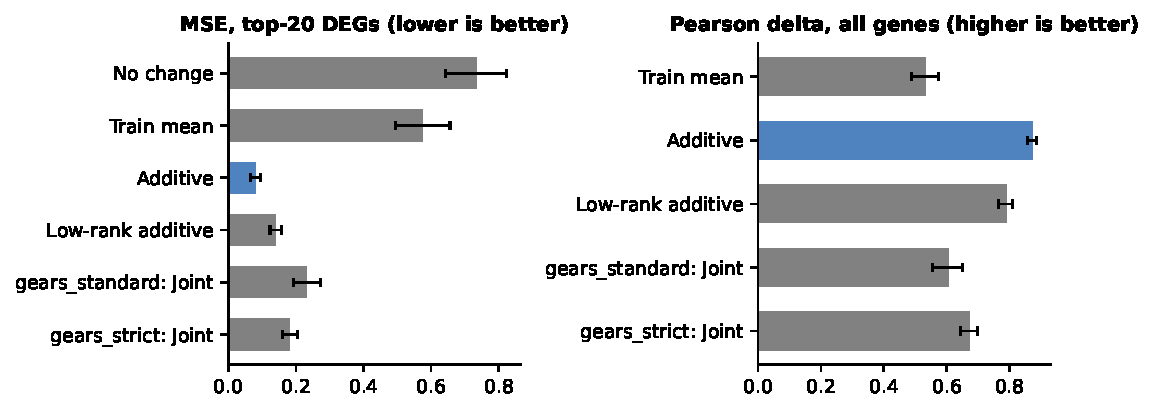
\includegraphics[width=\linewidth]{figs/fig2_null_hierarchy.pdf}
\caption{Baselines and GEARS joint prediction on held-out doubles, with 95\% bootstrap
intervals. Addition (blue) has the lowest error and the highest \pd.}
\label{fig:hier}
\end{figure}

GEARS is scored on fewer pairs for two reasons. Three doubles contain a gene outside GEARS's
gene-ontology graph (IER5L+LYL1, RHOXF2BB+SET, RHOXF2BB+ZBTB25), and on its standard split
GEARS also trains on 57 doubles, which are excluded. On the same pairs, addition scores
0.082 (128 pairs) and 0.085 (71 pairs), so the gap is not a pair-set artefact. On the strict
split, GEARS's MSE exceeds addition's by 0.100 [0.077, 0.122], and GEARS is better on only
14\% of pairs; on the standard split the gap is 0.148 [0.106, 0.187], with GEARS better on
13\%. The two GEARS rows are not directly comparable, because the standard set includes
pairs with a single never seen in training.

\noindent\textbf{Non-additivity is a reproducible property of each pair.} $\eta$ measured on
two disjoint cell halves agrees with Spearman 0.944 (per seed 0.932 to 0.955;
\Cref{fig:eta}). The cross-half estimate of true $\eta^2$ is positive for 99.5\% of pairs
and accounts for 61\% of measured $\eta^2$, so $\eta$ is mostly signal, with a noise share
of about 40\%.

\begin{figure}[htb]
\centering
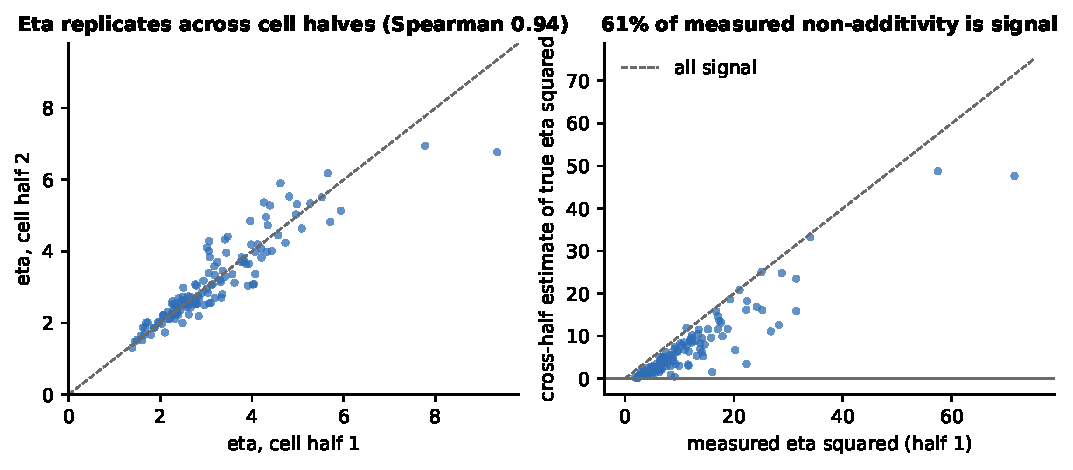
\includegraphics[width=\linewidth]{figs/fig1_eta_reliability.pdf}
\caption{Non-additivity replicates across disjoint cells. Left: $\eta$ on cell half 1 vs.\
half 2. Right: cross-half estimate of true $\eta^2$ vs.\ measured $\eta^2$; the dashed line
is ``all signal''.}
\label{fig:eta}
\end{figure}

\noindent\textbf{Additive error rises with non-additivity.} With $\eta$ from half 1 and error
from half 2, $\eta$ and additive MSE correlate with Spearman 0.82 across pairs
(\Cref{fig:addeta}). Additive error rises about fivefold from the low to the high tertile;
GEARS stays above it throughout, and the gap narrows only where interactions are strongest
(\Cref{tab:tert}). The most non-additive pairs are dominated by the CEBP family
(CEBPA+CEBPB, CEBPA+CEBPE, CEBPE+SET, CEBPA+KLF1), consistent with the redundant
differentiation programmes Norman et al.\ described.

\begin{figure}[htb]
\centering
\begin{minipage}{0.52\linewidth}
\centering
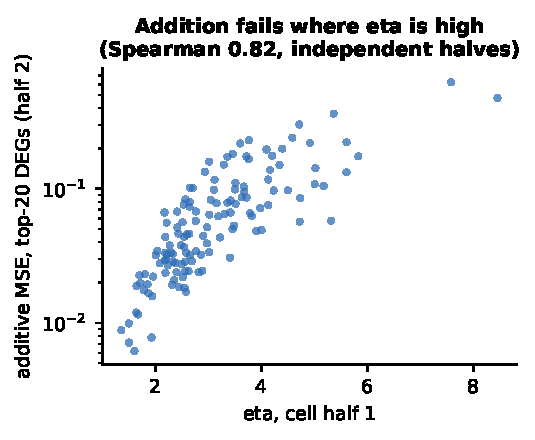
\includegraphics[width=\linewidth]{figs/fig3_additive_vs_eta.pdf}
\captionof{figure}{Additive error (half 2) against $\eta$ (half 1), one point per double.}
\label{fig:addeta}
\end{minipage}\hfill
\begin{minipage}{0.44\linewidth}
\centering
\small
\begin{tabular}{lcc}
\toprule
$\eta$ tertile & Additive & GEARS strict \\
\midrule
Low & 0.028 & 0.140 \\
Mid & 0.064 & 0.210 \\
High & 0.153 & 0.194 \\
\bottomrule
\end{tabular}
\captionof{table}{MSE on the top-20 DEGs by $\eta$ tertile, same 128 doubles. GEARS is worse
than addition in every tertile.}
\label{tab:tert}
\end{minipage}
\end{figure}

\noindent\textbf{Round-trip gate.} Strict GEARS passes on the 5 singles with the most cells
(KLF1, BAK1, CEBPE, ETS2, UBASH3B). Real $A$-perturbed cells passed through with no new
perturbation come back with $r = 0.999$ on expression and 0.80 to 0.99 on shifts from
control, and its own predicted states behave the same. The pass is structural, not learned:
a second application of $A$ moves the cell exactly as far as the first, so the shift simply
doubles (saturation ratio 1.0 for all five genes). The GEARS source explains why: input expression enters only as a final
residual, $\mathrm{out} = x + g(\mathrm{pert})$, and $g$ ignores the input cell.


\section{Analysis and Ablations}
\label{sec:analysis}
The midterm results already answer RQ1 for GEARS (it does not beat addition) and reduce RQ2
for GEARS to a comparison of two additive constructions.

\noindent\textbf{$\eta$ is reproducible across cells.} The worry was that ``highly
non-additive'' pairs might just be the noisiest ones, making their high error a
regression-to-the-mean artefact. The split-half design rules this out: $\eta$ replicates
across disjoint cells (Spearman 0.94), and every error is scored on the half not used to
define the groups. Reproducibility alone does not show that $\eta$ measures interaction rather than perturbation
size; the caveat at the end of this section addresses that. The high-$\eta$ tertile is where a
model with real interaction knowledge has room to beat addition.

\noindent\textbf{Addition is a hard bar, and the room above it is concentrated.} Most of
addition's error sits in the top $\eta$ tertile, five times the low tertile's. An overall
average therefore mostly reflects easy, near-additive pairs, so the rollout analysis will
report advantage over addition as a function of $\eta$, not as one average.

\noindent\textbf{Ablation: smoothing the singles does not help.} Low-rank addition is worse
than plain addition on 82\% of pairs. With pseudobulks from roughly 100 to 300 cells, the
single effects are already precise, so the rank-10 projection removes more real signal than
noise. A singles-only model must know something about how effects interact to beat addition.

\noindent\textbf{GEARS has not learned interactions, and it cannot carry state.} On the
strict split, GEARS's error exceeds addition's in every tertile; its gap narrows in the high
tertile (0.194 vs.\ 0.153) but does not reverse. Its predicted shift also ignores the input
cell, so its rollouts are fixed by construction:
\begin{equation}
\text{carried: } x + g(A) + g(B), \qquad \text{restated: } x + g(A) + g(A,B).
\end{equation}
The carried rollout cannot depend on order, since $g(A) + g(B)$ is symmetric. The
restated rollout can: it equals the joint prediction plus an extra $g(A)$, so it counts $A$
twice and should overshoot GEARS's joint prediction by exactly $g(A)$. Applying $A$ twice
simply doubles its shift. For GEARS, the remaining empirical question is whether its own
singles, $g(A) + g(B)$, land closer to the measured double than its joint $g(A,B)$. Because
$g(A)$ is trained to match each measured single, we expect the carried rollout to score
close to the \addnull, and so better than GEARS's joint prediction; that would reflect
addition, not composition. scGPT takes input expression by design, so composition is an open question for it; the
round-trip gate will test whether its output actually depends on its input.

\noindent\textbf{Caveat: $\eta$ partly tracks effect size.} $\eta$ correlates with the size
of the double's shift (Spearman 0.54), and shift size alone predicts additive error about as
well (0.58). $\eta$ relative to the shift barely predicts it (0.15), and the scale-free \pd
hardly falls across tertiles (0.880 to 0.862). Part of the trend is ``bigger perturbations
have bigger absolute errors''. For the final report we will compare models with addition
within tertiles, which cancels scale, and check conclusions with relative $\eta$ or effect
size as a covariate.


\section{Limitations}
\label{sec:limitations}
The midterm results rest on one dataset, one GEARS seed and joint predictions only.
\begin{itemize}[nosep]
  \item \textbf{One dataset.} Norman is the only public set with doubles and all their
  singles, so we cannot test generality on another cell type or perturbation modality.
  \item \textbf{Biology of rollout.} Norman's guides act together for the whole experiment.
  Neither rollout arm matches that exactly, and order and saturation cannot be validated
  biologically.
  \item \textbf{One GEARS run.} Each regime was trained once (seed 1, 20 epochs, default
  hyperparameters); seed-to-seed variation and tuning are untested.
  \item \textbf{Unpredictable pairs.} GEARS cannot perturb RHOXF2BB, KIAA1804 or IER5L, so 3
  of 131 doubles are missing from its scores.
  \item \textbf{Effect-size confound.} $\eta$ partly measures the size of the perturbation,
  not only its non-additivity (\Cref{sec:analysis}).
  \item \textbf{One model can test composition.} GEARS's rollout is additive by
  construction, so the composition question (RQ2) rests on scGPT alone.
  \item \textbf{Rollout not yet run.} The midterm reports joint predictions only; the
  composition results are still to come.
\end{itemize}


\section{Timeline for Remaining Work}
\label{sec:timeline}
The full rollout experiment runs next; by November 15 we decide whether scGPT passes the
round-trip gate or the study proceeds with GEARS alone (\Cref{tab:timeline}).

\begin{table}[htb]
\centering
\small
\begin{tabularx}{\linewidth}{llX}
\toprule
By & Owner & Work \\
\midrule
Nov 15 & Shreyan & Full rollout on strict GEARS: both arms, both orders, measured-input control \\
Nov 15 & Shreyan & Standard-split GEARS rollout as the diagnostic comparison \\
Nov 15 & Shreyan & scGPT adapter and round-trip gate; joint and rollout only if it passes \\
Nov 15 & Datta & Rollout analysis: advantage over addition vs.\ $\eta$ (slope + CI), order dependence, arm comparison \\
\midrule
Nov 15 & Both & \textbf{Decision: keep scGPT, or GEARS only} \\
\midrule
After Nov 15 & Datta & Stability: saturation ratio and drift from real cells over 1 to 10 steps \\
After Nov 15 & Datta & Effect-size checks: within-tertile comparisons and relative $\eta$ \\
Nov 22 & Both & Draft final-report figures \\
Dec 3 & Both & Final report and presentation \\
\bottomrule
\end{tabularx}
\caption{Plan for the remaining work. If time runs short we cut, in order: the
discriminator-based drift metric, five split seeds down to three, scGPT, and the stability
experiment.}
\label{tab:timeline}
\end{table}


\clearpage
\printbibliography

\end{document}
